%%%%%%%%%%%%%%%%%%%%%%%%%%%%%%%%%%%%%%%%%%%%%%%%%%%%%%%%%%%%%%%%%%%%%%%%%%%
%% This file is part of the book
%%
%% Algorithmic Graph Theory
%% http://code.google.com/p/graph-theory-algorithms-book/
%%
%% Copyright (C) 2009, 2010, 2011 Minh Van Nguyen <nguyenminh2@gmail.com>
%%
%% See the file COPYING for copying conditions.
%%%%%%%%%%%%%%%%%%%%%%%%%%%%%%%%%%%%%%%%%%%%%%%%%%%%%%%%%%%%%%%%%%%%%%%%%%%

\subfigure[]{
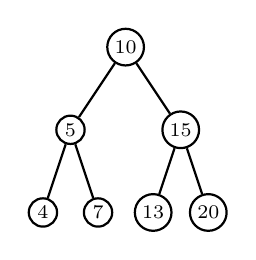
\begin{tikzpicture}
[-,thick,%
  every node/.style={shape=circle,inner sep=1.5pt,draw,thick},%
  scale=0.7]
\scriptsize
\node {$10$}
  [sibling distance=2cm]
  child {node {$5$}
    [sibling distance=1cm]
    child {node {$4$}}
    child {node {$7$}}
  }
  child {node {$15$}
    [sibling distance=1cm]
    child {node {$13$}}
    child {node {$20$}}
  };
\end{tikzpicture}
}
%%
%%
\qquad
\subfigure[]{
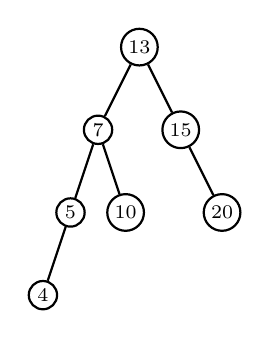
\begin{tikzpicture}
[-,thick,%
  every node/.style={shape=circle,inner sep=1.5pt,draw,thick},%
  scale=0.7]
\scriptsize
\node {$13$}
  child {node {$7$}
    [sibling distance=1cm]
    child {node {$5$}
      child {node {$4$}}
      child[missing]
    }
    child {node {$10$}}
  }
  child {node {$15$}
    child[missing]
    child {node {$20$}}
  };
\end{tikzpicture}
}
%%
%%
\qquad
\subfigure[]{
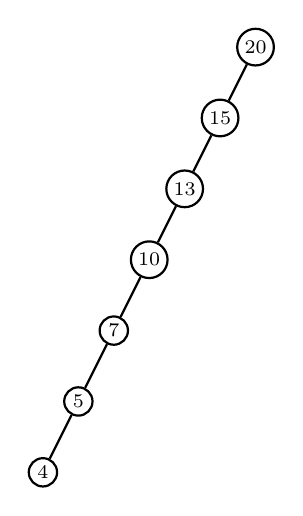
\begin{tikzpicture}
[-,thick,%
  every node/.style={shape=circle,inner sep=1.5pt,draw,thick},%
  scale=0.6]
\scriptsize
\node {$20$}
  child {node {$15$}
    child {node {$13$}
      child {node {$10$}
        child {node {$7$}
          child {node {$5$}
            child {node {$4$}}
            child[missing]
          }
          child[missing]
        }
        child[missing]
      }
      child[missing]
    }
    child[missing]
  }
  child[missing];
\end{tikzpicture}
}
%%
%%
\qquad
\subfigure[]{
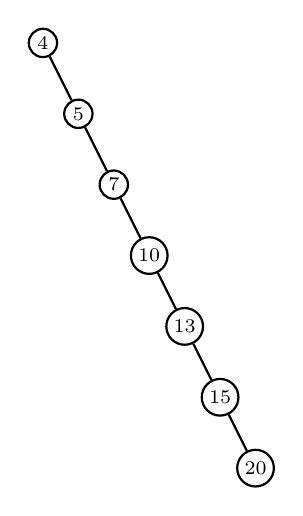
\begin{tikzpicture}
[-,thick,%
  every node/.style={shape=circle,inner sep=1.5pt,draw,thick},%
  scale=0.6]
\scriptsize
\node {$4$}
  child[missing]
  child{node {$5$}
    child[missing]
    child {node {$7$}
      child[missing]
      child {node {$10$}
        child[missing]
        child {node {$13$}
          child[missing]
          child {node {$15$}
            child[missing]
            child {node {$20$}}
          }
        }
      }
    }
  };
\end{tikzpicture}
}
